% !TeX TS-program = XeLaTeX
% check for outdated packages, syntax etc.
\RequirePackage[l2tabu,orthodox]{nag}

\documentclass[a4paper,12pt]{article}

% polyglossia should go first!
\usepackage{xltxtra} % for XeLaTeX logo ^_^
\usepackage{polyglossia} % multi-language support
 
\usepackage{amsmath} % math symbols, new environments and stuff
\usepackage{unicode-math} % for changing math font and unicode symbols
\usepackage[style=english]{csquotes} % fancy quoting
\usepackage{microtype} % for better font rendering
\usepackage[backend=biber]{biblatex} % for bibliography
\usepackage{hyperref} % for refs and URLs
\usepackage{graphicx} % for images (and title page)
\usepackage{geometry} % for margins in title page
\usepackage{tabu} % for tabulars (and title page)
\usepackage{placeins} % for float barriers
\usepackage{titlesec} % for section break hooks
\usepackage{totcount} % total count of things
% \usepackage{cleveref} % ref auto-naming (doesn't support polyglossia)
%\usepackage[justification=centering]{caption} % for forced captions centering
\usepackage{subcaption} % for subfloats
%\usepackage{rotating} % for rotated labels in tables
\usepackage{tikz} % for TiKZ
%\usepackage{dot2texi} % for inline dot graphs
\usepackage{listings} % for listings 
%\usepackage{upquote} % for good-looking quotes in source code (used for custom languages)
\usepackage{multirow} % for multirow cells in tabulars
%\usepackage{afterpage} % for nice landspace floats and longtabus
%\usepackage{pdflscape} % for landspace orientation
\usepackage{xcolor} % colors!
%\usepackage{enumitem} % for unboxed description labels (long ones)
%\usepackage{numprint} % pretty-printing numbers
%\usepackage{longtable} % for longtabu

\setmainlanguage{russian}
\setotherlanguage{english}
\defaultfontfeatures{Mapping=tex-text} % for converting "--" and "---"
\setmainfont{CMU Serif}
\setsansfont{CMU Sans Serif}
\setmonofont{CMU Typewriter Text}
\setmathfont{XITS Math}
\DeclareSymbolFont{letters}{\encodingdefault}{\rmdefault}{m}{it} % for Russian in math
%\MakeOuterQuote{"} % enable auto-quotation

% new page and barrier after section, also phantom section after clearpage for
% hyperref to get right page.
% clearpage also outputs all active floats:
\newcommand{\sectionbreak}{\FloatBarrier\newpage\phantomsection}
%\newcommand{\subsectionbreak}{\FloatBarrier}
\renewcommand{\thesection}{\arabic{section}} % no chapters
\numberwithin{equation}{section}
\renewcommand{\figurename}{Рисунок} % Russian standards

%\usetikzlibrary{shapes,arrows,trees}
\usetikzlibrary{positioning}
\pgfmathsetmacro{\mylinesep}{0.2cm}
\tikzset{
  bitbox/.style={
    draw,
    inner sep=2,
    outer sep=0,
    minimum height=\heightof{ABC}+2*2*1mm,
    align=center
  }
}

\lstset{
  language=Haskell,
  numbers=left,
  numberstyle=\scriptsize,
  basicstyle=\ttfamily\scriptsize,
  columns=fullflexible,
  keepspaces, % for spaces in unicode text!
  captionpos=b % Russian standards, again
}
\renewcommand{\lstlistingname}{Листинг}

%\newcommand{\un}[1]{\: \mathit{#1}} % unit measurements

\newcounter{refs} % count total number of references

\makeatletter
\let\thetitle\@title
\let\theauthor\@author
\let\thedate\@date

\defbibenvironment{counter}
  {\setcounter{refs}{0}
   \renewcommand{\blx@driver}[1]{}}
  {}
  {\stepcounter{refs}}
\defbibheading{counter}{}
\makeatother

\addglobalbib{summary.bib}

\title{Диплом}
\author{Амиантов Н.И., ИУ7-82}
\date{\today}

\begin{document}

\tableofcontents
\newpage

\section*{Реферат}
Дипломная работа, \regtotcounter{page}\total{page} стр.,
\regtotcounter{figure}\total{figure} рис., \regtotcounter{table}\total{table}
таб., \regtotcounter{refs}\total{refs} источников.

Ключевые слова: хранение изображений, сжатие с потерями, выбор палитры,
квантизация, ошибка сжатия

Объект исследования: возможные способы сжатия изображений при помощи
динамического выбора уровня сжатия для различных блоков.

Цель: получение нового метода сжатия изображений с потерями, основанного на
динамическом выборе сжатия. Нахождение алгоритмов, пригодных для подобного
сжатия.

Методы исследования: изучение существующих алгоритмов, визуальные эксперименты с
различными параметрами сжатия, сравнение различных метрик ошибки сжатия.

В результате проведённого исследования были найдены оптимальные параметры и
алгоритмы сжатия для построенного формата изображения. Найдено, что лучше всего
ведёт себя для сжатия изображений в среднем метрика, основанная на идее
нахождения пространственных серий в блоках изображения. Изучены различные
алгоритмы улучшения качества изображения с уменьшенной палитрой. Установлено,
что алгоритм распостранения ошибки улучшает визуально изображение, сжатое в
описанном формате, и найдена оптимальная матрица обхода для
алгоритма. Найден оптимальный алгоритм нахождения палитры для одного канала
изображения в усновиях заданного числа элементов. Найден алгоритм нахождения
оптимального уровня сжатия блока изображения, основанный на найденной метрике
ошибки сжатия.

\section*{Введение}

Алгоритмы сжатия изображений в той или иной форме, с потерями качества и без, и
с разными областями применения используются для уменьшения занимаемого
изображением пространства уже достаточно давно. Существует несколько известных
подходов к сжатию изображений, алгоритмов и вспомогательных шагов. Мы
представляем новый метод сжатия изображений, основанный на сжатии палитры,
обладающий полезным набором свойств.

\section{Аналитический раздел}

\subsection{Введение}

Перед заданием нового формата необходимо рассмотреть существующие решения,
классифицировать их по областям применения, рассмотреть их достоинства и
недостатки. Также в этом разделе мы рассмотрим известные популярные алгоритмы,
используемые в сжатии изображений.

\subsection{Задача}

Необходимо разработать формат хранения изображений с потерями и алгоритмы сжатия и
распаковки для преобразования изображений в этот формат. Считается, что исходные
изображения представлены в несжатом растровом виде, т.е. как массивы байт,
обозначающих интенсивность каждого канала изображения. Исходные изображения
могут быть представлены одним каналом яркости (изображения в оттенках серого)
или как сумма трёх каналов красного, зелёного и синего цветов. Изображение после
расшифровки должно быть представлено в схожем формате. Пользователю
предоставляется возможность влиять на параметры сжатия. Некоторые параметры
сжатия могут быть заданы в описании формата заранее, другие должны содержаться в
конечном сжатом файле с целью восстановления исходной картинки. Подразумевается,
что алгоритм сжатия не используется для сжатия видео, а значит не создан для
сжатия и распаковки в реальном времени, так что в процессе работы программы
могут быть использованы более ресурсоёмкие, но дающие лучший результат
алгоритмы.

\subsection{Описание предметной области}

Существует несколько известных классов алгоритмов сжатия изображений. В первую
очередь, следует различать области, для которых применяется сжатие, и возможные
свойства алгоритмов.

\subsubsection{Векторные и растровые изображения}

Изображения могут быть представлены как в форме прямоугольной матрицы
интенсивностей (растровый вид) и математического описания составляющих в виде
уравнений (векторный вид). Для векторных изображений существует отдельный класс
алгоритмов работы с ними, и они не попадают в область данной статьи. В
дальнейшем в статье под ``изображениями'' будут пониматься именно растровые изображения.

\subsubsection{Сжатие с потерями и без потерь}

Для некоторых классов изображений важно отсутствие потерь любых деталей по
сравнению с оригиналом. Такие требования обязательны для хранения медицинских
изображений (фотографий, результатов исследований), научных изображений
(результаты экспериментов, напр., фотографии с электронных микроскопов), в том
числе астрономических фотографий. Также сжатие без потерь используется для
сжатия изображений, составляющих графический интерфейс пользователя, например
частей оформлений веб-сайтов, иконок приложений, структурных элементов интерфейса.

Сжатие с потерями используется для любительской и большей части профессиональной
фотографии, передачи изображений по сети Интернет, архивации изображений в
условиях ограниченного дискового пространства. В области сжатия видео
применяются алгоритмы, комбинирующие выявление т.н. ``ключевых кадров'' и
отличий между ними и последующими кадрами с сжатием ключевых кадров (и таких
отличий) алгоритмами сжатия изображений с потерей данных.~\cite{wiki:mpeg}
Сжатие с потерями также может использоваться для сжатия сканированных
документов, которые к тому же обладают особой спецификой (напр., уменьшенной
цветовой гаммой, особенно в случае книг). Разработанный алгоритм относится к
классу алгоритмов сжатия с потерями.

\subsubsection{Форма работы с изображением}

Изображение можно рассматривать с нескольких позиций. В первую очередь следует
отметить, что изображение представляет собой двумерный дискретный сигнал, и к
нему применимы обычные алгоритмы преобразования двумерных сигналов. Также
изображения могут быть представлены как набор одномерных дискретных сигналов,
если применять к ним некую форму развёртки (по строкам, по столбцам или более
сложные формы), и в такой форме также могут обрабатываться. Большинство форматов
использует комбинацию обработки изображения как одномерного развёрнутого сигнала
и как двумерного. Например, известный формат JPEG использует разделение
изображения на блоки 8х8 и работает с ними как с матрицами, а затем сжимает
изображение как поток байт.~\cite{jpeg}.

\subsubsection{Класс алгоритмов}

Для сжатия изображений используется несколько классов алгоритмов, применяемых
раздельно или в комбинации. Это алгоритмы сжатия палитры, преобразование Фурье с
различными базисами и вейвлет-преобразования, алгоритмы предугадывания
пикселей на основе окружающих, Про наиболее популярные алгоритмы будет
рассказано далее.

\subsubsection{Особенности сжатия}

Как следствие применения конкретных алгоритмов, различные форматы обладают
различными особенностями по отношению к разным типам изображений. Например,
формат JPEG хорошо сжимает фотографии и подобные изображения, PNG подходит для
элементов интерфейса с чёткими границами, DjVu -- для сжатия сосканированных
книг и пр.

\subsubsection{Цветовые палитры}

Если изображение должно содержать информацию о цвете, то оно должно хранить её в
заранее известной системе координат для цветов. Наиболее известной подобной
системой координат является \emph{RGB}, в которой для задания цветовой точки
используется три координаты -- яркости красной, зелёной и синей составляющей в
ней. Эта система координат удобна из-за особенностей технологий, применяемых в
современных дисплеях, в которых точки представлены тремя близко расположенными
субпикселями этих трёх цветов. Также такой формат удобен при печати --
печатающие устройства используют смешение красок для получения нужного цвета, и
RGB -- один из вариантов исходных наборов таких красок. Однако работать с таким
изображением, будь то сжатие или просто обработка, неудобно из-за
неинтуитивности отношения яркости и тона. Существует два основных класса палитр
-- типографские, используемые при печати и отображении (к которым относится и
RGB), и палитры схожие с \emph{YUV}, в которых цвет представлен отдельной
яркостной составляющей и координатами в цветовом пространстве, не зависящем от
яркости. Известной палитрой такого рода является цветовое пространство
\emph{Lab}~\cite{lab}, которое охватывает все наблюдаемые цвета и
используется как наиболее общая и независящая от аппаратных особенностей
палитра. С точки зрения алгоритмов сжатия второй класс палитр более
предпочтителен, т.к. из-за особенностей человеческого глаза цветовую
составляющую можно сжимать сильнее, чем яркостную.

\subsubsection{Дополнительные возможности}

Форматы хранения изображений могут включать в себя дополнительные полезные
возможности. Например, формат может содержать в себе дополнительную информацию
об изображении, как то: время и место создания, настройки фотокамеры в случае
фотографии, сведения об авторе и правах распостранения.

Достаточно популярной дополнительной возможностью многих форматов,
ориентированных на использование в сети Интернет и для изображений-элементов
пользовательского интерфейса является хранение информации о прозрачности точек
изображения, позволяющая накладывать изображения друг на друга и создавая таким
образом целостный вид. Например, такая возможность может использоваться для игр,
использующих спрайты (напр., Doom~\cite{wiki:doom}) для отделения элементов фона
от собственно спрайтов (персонажей и.т.д.).

Ещё одной популярной воможностью является хранение информации об изображении в
определённом порядке, позволяющем показывать изображение по мере загрузки
сначала в общих деталях,а затем со всё растущим уровнем детализации. Эту
возможность поддерживают все популярные форматы, используемые в сети интернет --
PNG, JPEG и GIF~\cite{png}\cite{jpeg}\cite{gif}, используя разные механизмы
хранения данных в таком виде.

Наконец, известной особенностью форматов GIF и PNG является поддержка анимации,
из-за которой они пользуются большой популярностью в сети Интернет.

\subsection{Требования к формату}

Исходя из описания предметной области, можно предложить составить список
требований к новому формату, которые будут определять выбираемые алгоритмы.

\begin{itemize}
\item Формат будет использовать сжатие с потерями данных;
\item Формат будет использоваться для сжатия статических изображений;
\item Формат будет разрабатываться для сжатия фотографических изображений, но с
  сохранением границ, позволяющем использовать его для сканированных книг и текстов.
\end{itemize}

Далее мы рассмотрим известные алгоритмы сжатия изображений (исключая форматы)
подробнее.

\subsection{Алгоритмы сжатия изображений}

Алгоритмы сжатия можно разделить на основные и вспомогательные. К основным
алгоритмам мы относим те, основной смысл которых состоит именно в уменьшении
размера изображения. К вспомогательным отнесём те, которые улучшают качество
сжатого изображения, добавляют дополнительные возможности и
прочее. Рассматривать алгоритмы мы будем по этапам, в которых они применяются.

\subsubsection{Изменение цветовой палитры}

В большом количестве форматов сжатия данных используется палитра $YC_bC_r$, вариации
которой используются также для передачи телесигнала. Существует несколько
вариаций этой палитры -- свои варианты с небольшими изменениями используются в
традиционной телетрансляции, HDTV и в сжатии изображений~\cite{palettes}. Для
этих применених характерны разные области, в которых задано цветовое
пространство, и его ``охват'' цветов. В области сжатия изображений популярностью
пользуется вариация из стандарта JFIF~\cite{jfif}, используемая с алгоритмом
сжатия JPEG. Эта цветовая палитра позволяет удобнее работать с
изображением, в частности, применяя более агрессивное сжатие к цветовой
составляющей -- для человека это менее заметно, чем сжатие яркостной.

\subsubsection{Сжатие палитры}

Для лучшего сжатия применяют сокращение возможных цветового и яркостного
диапазонов. Редкие изображения используют одновременно все им доступные цвета;
важным исключением являются фотографии, где сложно выбрать однозначный набор
необходимых цветовю. Сложность сжатия в основном состоит из двух проблем --
выбора количества цветов и поиск оптимальных значений для них. Для поиска
палитры в целом подходит любой алгоритм многомерной кластеризации. Существуют
специализированные алгоритмы выбора цветов для палитры,
напр.,~\cite{leptonica:colorquant}. После выбора оптимальных значений цвета
назначаются в соответствии с оптимальной на данном цветовом пространстве
метрикой расстояния. В этом смысле выделяется цветовое пространство \emph{Lab},
в котором эвклидова метрика расстояния достаточно точно коррелирует со степенью
различия цветов, наблюдаемой человеком.

Количество цветов в будущей палитре, во всяком случае, максимальное, часто
фиксировано в формате данных. Повторяющееся цвета из палитры обычно удаляются.

\subsubsection{Выделение блоков}

Эта ступень может проходить на разных этапах сжатия и служит для разделения
изображения на отдельные участки, с которыми будет в дальнейшем продолжаться
работа. Блоки выбираются целесообразно алгоритму, которым их в дальнейшем будут
сжимать. Блоки могут также применяться просто для разделения изображения --
напр., в стандарте JPEG-2000 изображение определено как набор произвольных
прямоугольных блоков, которых могут быть обработаны отдельно. 

\subsubsection{Преобразование вида хранения изображения}

Это достаточно обширная категория, включающая в себя в частности два наиболее
известных метода сжатия изображений -- дискретное косинусное преобразование
(DST) и дискретное вейвлет-преобразование (DWT). Первое используется в частности
в алгоритме сжатия изображений JPEG~\cite{jpeg}, тогда как второе -- в его
наследнике JPEG-2000, протоколе передачи удалённого рабочего стола RDP (а
именно, в кодеке передачи картинки RemoteFX~\cite{remotefx}) и.т.д. На больших
изображениях DWT даёт значительное преимущество перед DST, и используется в
основном в современных форматах сжатия изображений с потерями. Оба метода
позволяют получить другое представление изображения (обычно, с потерей данных),
которое позволяет хранить данные более компактно. Мы рассмотрим оба популярных
метода.

\paragraph{Дискретное косинусное преобразование}
Это преобразование используется в алгоритме сжатия изображений JPEG. Идея
состоит в преобразовании исходной матрицы в линейную комбинацию некоторого
заранее известного базиса. Пример базиса (для JPEG) приведён на
рисунке~\ref{fig:jpegbas}. Затем малозначащие коеффициенты отбрасываются из
результирующего выражения. Таким образом достигается сжатие.

\begin{figure}
  \centering
  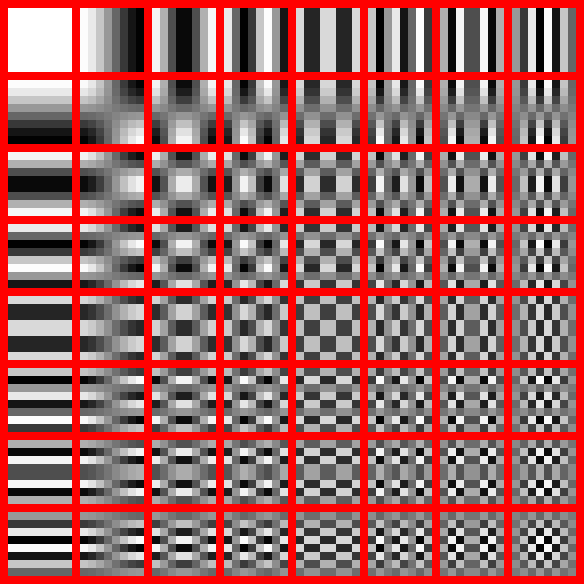
\includegraphics[width=0.9\textwidth]{img/dctjpeg}
  \caption{Базис JPEG для DCT}
  \label{fig:jpegbas}
\end{figure}

\paragraph{Дискретное вейвлет-преобразование}
Вейвлет-преобразование -- это альтернатива DST в более современных
алгоритмах. Вейвлет-преобразование выгодно отличается от DST тем, что оно
позволяет хранить информацию в двух измерениях -- не только о частоте, но и о
позиции.~\cite{jour:wavelets}. Вейвлет-преобразование производится в несколько
рекурсивных этапов, на каждом из которых изображение разделяется на
``подробности'', хранящие информацию, позволяющую увеличить разрешение
изображения, и само изображение в уменьшенном виде.

\subsubsection{Линеаризация}

В конечном итоге изображение хранится как последовательность интенсивностей, так
что для него должен быть применён какой-то алгоритм линеаризации --
обратимого преобразования двумерной матрицы в конечную последовательность. Сами
по себе способы обхода матрицы тривиальны, однако определённые методы обхода
могут использоваться для прогрессивного кодирования, т.е. когда изображение
загружается от общего к деталям по мере поступления данных. Такие методы обхода
также известны как алгоритмы интерлейсинга. Для такого обхода существуют
несколько схем; одна из наиболее продвинутых используется в формате PNG --
алгоритм \emph{Adam7}. Для декодирования изображений с использованием таких
алгоритмов обычно применяют интерполяцию (напр., бикубическую) для лучшего
визуального эффекта.

На этапе линеаризации также может применяться разностное кодирование.

\subsubsection{Сжатие последовательности}

На этом этапе применяются алгоритмы сжатия без потерь -- специализированные для
изображений или общего применения. Из наиболее часто применяемых алгоритмов
общего применения выделяется LZW, используемый в форматах GIF и PNG, а также
кодирование Хаффмана, применяемое в JPEG и EBCOT, который иcпользуется в JPEG-2000.

\subsection{Вывод}

Мы описали необходимые требования к будущему формату и алгоритму сжатия
изображений, а также рассмотрели известные популярные алгоритмы, используемые в
сжатии изображений.

\section{Конструкторский раздел}

\subsection{Введение}

Предложенный нами формат использует идею, которая не применялась до сих пор в
обычных форматах сжатия изображений -- динамический выбор палитры и степени
сжатия для каждого блока по отдельности, и разбиение блоков на подблоки со своей
палитрой. Мы собираемся задать формат файла и необходимых структур в памяти, а
также описать алгоритм сжатия без указания конкретных способов выполнения
некоторых этапов (которые могут быть выбраны несколькими способами и изучались в
исследовательской части).

\subsection{Общая структура}

Общая структура формата показана в листинге~\ref{lst:bakaimage}. Заголовок
формата содержит информацию о размере изображения и список каналов, о которых
будет сказано ниже. Структура формата в бинарном виде представлена на
рисунке~\ref{fig:bakaimage}. В бинарном представлении добавляется общее
количество каналов в файле.

\begin{lstlisting}[float=t,caption={Основной заголовок формата},label=lst:bakaimage]
  data ChannelType = Y | Cb | Cr

  type Size = (Word64, Word64)

  data BakaImage = BakaImage Size [(ChannelType, Channel)]
\end{lstlisting}

\begin{figure}[t]
  \centering
  \begin{tikzpicture}[scale=0.7, transform shape]
    \draw[thick,->] (0,0) -- (20,0) node[anchor=north east] {б};
    \foreach \x in {0,8,16,17}
      \draw (\x cm,1pt) -- (\x cm,-1pt) node[anchor=north] {$\x$};
    \node[bitbox,minimum width=8cm,above right,yshift=\mylinesep](1) {Высота};
    \node[bitbox,minimum width=8cm,right=0cm of 1](2) {Ширина};
    \node[bitbox,minimum width=1cm,right=0cm of 2](3) {№};
    \node[right=0cm of 3] {Каналы...};
  \end{tikzpicture}
  
  \caption{Заголовок формата}
  \label{fig:bakaimage}
\end{figure}

Дальшейшие структуры формата будут рассматриваться одновременно с алгоритмами,
используемыми для кодирования изображения.

\subsection{Предварительные преобразования}

На первых этапах изображение должно быть преобразовано к палитре
$YC_bC_r$. Матрицы преобразований из $RGB$ в эту цветовую палитру и наоборот
представлены в таблице~\ref{tab:yuv}.

\begin{figure}
  \centering
  \begin{subfigure}[b]{\textwidth}
    \[
    \begin{bmatrix}
      Y \\
      C_b \\
      C_r \\
    \end{bmatrix}
    =
    \begin{bmatrix}
      0 \\
      180 \\
      180 \\
    \end{bmatrix}
    +
    \begin{bmatrix}
      0.299 & 0.587 & 0.114 \\
      -0.1687 & -0.3313 & 0.5 \\
      0.5 & -0.4187 & 0.0813 \\
    \end{bmatrix}
    \times
    \begin{bmatrix}
      R \\
      G \\
      B \\
    \end{bmatrix}
    \]
    \caption{Из $RGB$ в $YC_bC_r$}
  \end{subfigure} \\
  \begin{subfigure}[b]{\textwidth}
    \[
    \begin{bmatrix}
      R \\
      G \\
      B \\
    \end{bmatrix}
    =
    \begin{bmatrix}
      1 & 0 & 1.402 \\
      1 & -0.34414 & -0.71414 \\
      1 & 1.772 & 0 \\
    \end{bmatrix}
    \times
    \begin{bmatrix}
      Y \\
      C_b - 128 \\
      C_r - 128 \\
    \end{bmatrix}
    \]
    \caption{Из $YC_bC_r$ в $RGB$}
  \end{subfigure}
  
  \caption{Преобразование в цветовую палитру $YC_bC_r$ и обратно}
  \label{tab:yuv}
\end{figure}

Для каждого канала изображение кодируется отдельно, со своими настройками
сжатия. Это позволяет детально настраивать процесс кодирования, ухудшая сжатие
цветовой составляющей и подстраивая настройки под разные типы
изображения. Описание структуры канала представлено в
листинге~\ref{lst:channel}. Заголовок канала состоит из его типа (составляющей,
которую он представляет) в строковом виде, например, ``Cb'', списка типов
блоков, которые могут содержаться в этом канале, и списка блоков изображения.  В
бинарном виде заголовки каналов изображения построены как показано на
рис.~\ref{fig:channel}. Количество типов блоков записывается в бинарном виде
отдельно, однако количество самих блоков не записывается -- оно вычисляемо из
информации о типах блоков и размере изображения.

\begin{lstlisting}[float=t,caption={Структура канала},label=lst:channel]
  data Channel = Channel [BlockInfo] [Block]
\end{lstlisting}

\begin{figure}[t]
  \centering
  \begin{tikzpicture}
    \draw[thick,->] (0,0) -- (10,0) node[anchor=north east] {б};
    \node[bitbox,,above right,yshift=\mylinesep](1) { Имя канала... };
    \node[bitbox,minimum width=1cm,right=0cm of 1](2) { № };
    \node[bitbox,right=0cm of 2](3) { Типы блоков... };
    \node[bitbox,right=0cm of 3](4) { Блоки... };
  \end{tikzpicture}
  
  \caption{Заголовок канала}
  \label{fig:channel}
\end{figure}

\subsection{Разбиение на блоки}

Для изображения задаётся несколько возможных режимов кодирования блоков. Общий
формат информации о блоке представлен в листинге~\ref{lst:blockinfo}. Основным
свойством блока является его размер -- в частности, размер наибольшего блока
будет использоваться для всех блоков первого уровня в изображении. Изображение
разбивается согласно этому размеру и каждый блок обрабатывается отдельно. Также
для каждого блока содержится битрейт (количество бит, затрачиваемое на каждую
полную интенсивность), размер пикселя (при применении масштабирования) и размер
палитры для данного режима кодирования. Для данных блоков и ниже применяется
битовое сжатие -- данные записываются без выравнивания по байтам. Из-за
особенностей кодирования это сильно влияет на размер изображения. Важным
параметром канала также является общее число возможных режимов кодирования,
которое влияет на длину поля типа блока у каждого блока канала. Бинарный формат
информации о блоке представлен на рисунке~\ref{fig:blockinfo}.

\begin{lstlisting}[float=t,caption={Структура информации о кодировании блока},label=lst:blockinfo]
  type SmallSize = (Word8, Word8)
  data BlockInfo = BlockInfo
    { levels :: Word8
    , sbsize :: SmallSize
    , pixel :: SmallSize
    , bitrate :: Word8
    }
\end{lstlisting}

\begin{figure}[t]
  \centering
  \begin{tikzpicture}
    \draw[thick,->] (0,0) -- (8,0) node[anchor=north east] {б};
    \foreach \x in {0,1,3,5,6}
      \draw (\x cm,1pt) -- (\x cm,-1pt) node[anchor=north] {$\x$};
    \node[bitbox,minimum width=1cm,above right,yshift=\mylinesep](1) {lvls};
    \node[bitbox,minimum width=2cm,right=0cm of 1](2) {sbsz};
    \node[bitbox,minimum width=2cm,right=0cm of 2](3) {px};
    \node[bitbox,minimum width=1cm,right=0cm of 3](4) {br};
  \end{tikzpicture}
  
  \caption{Информация о режиме кодирования}
  \label{fig:blockinfo}
\end{figure}

\subsection{Сжатие блоков верхнего уровня}

Формат использует два уровня блоков. Размер блоков верхнего уровня равен
наибольшему размеру блока в канале (как сказано выше). Все блоки второго уровня
(подблоки) внутри блока сжаты одинаковым способом. Формат блока верхнего уровня
представлен в листинге~\ref{lst:block}. В таком блоке содержится индекс режима
кодирования, который используется для всех подблоков. В бинарном представлении
индекс занимает минимальное количество места, исходя из количества возможных
режимов кодирования для данного канала. Затем такой блок хранит трёхмерный
массив интенсивностей и массив индексов, о которых будет рассказано
ниже. Бинарное представление блока верхнего уровня представлено на
рисунке~\ref{fig:block}.

При использовании уменьшения масштаба (пиксели размером больше 1х1) перед
обработкой матрица блока разбивается на блоки размером с будущие пиксели, и
формируется новая матрица, значения в которой равны средним значениям блоков
исходной.

\begin{lstlisting}[float=t,caption={Структура блока верхнего уровня},label=lst:block]
  data Block = Block Word8 (Array (Int, Int, Int) Word8) (Array (Int, Int) Word8)
\end{lstlisting}

\begin{figure}[t]
  \centering
  \begin{tikzpicture}
    \draw[thick,->] (0,0) -- (8,0) node[anchor=north east] {б};
    \node[bitbox,above right,yshift=\mylinesep](1) {Индекс уровня};
    \node[bitbox,minimum width=2cm,right=0cm of 1](2) {Интенсивности...};
    \node[bitbox,minimum width=2cm,right=0cm of 2](3) {Индексы...};
  \end{tikzpicture}
  
  \caption{Блок верхнего уровня}
  \label{fig:block}
\end{figure}

\subsection{Сжатие подблоков}

Блоки верхнего уровня бьются на подблоки согласно выбранному режиму
кодирования. Для каждого подблока имеется конечная последовательность в
трёхмерном массив интенсивностей, значения которой соответствуют $i$-ым
интенсивностям индивидуальной палитры подблока. Поскольку все подблоки сжимаются
с одним режимом кодирования, длины палитр для всех подблоков совпадают. Все
точки подблока сводятся к одному из значений индивидуальной палитры. Индексы
палитры хранятся побитово в зависимости от размера палитры, и подблоки хранятся
подряд, что обеспечивает высокую плотность информации.

\subsection{Последующее сжатие}

Каналы целиком сжимаются алгоритмом LZMA2, который обеспечивает дополнительное
сжатие. Такая обработка обеспечивает дальнейшее уменьшение объёма до 30\% от
исходной уже сжатой картинки.

\subsection{Раскодирование}

Раскодирование такого формата -- достаточно быстрая операция, не требующая
больших объёмов оперативной памяти или сложных вычислений. Основная
вычислительная операция -- распаковка сжатых алгоритмом LZMA2 каналов. После
распаковки достаточно считывать блоки подряд и заполнять матрицу будущих
интенсивностей поблочно. Размеры блоков известны до их считывания. Во время
чтения подблоков значения индексов подменяются в конечном раскодированном
изображении на значения из палитры. Полная схема раскодирования формата
представлена на рисунке~\ref{fig:unpack}.

\begin{figure}
  \includegraphics[width=0.9\textwidth,page=1]{img/unpack}
  \caption{Схема алгоритма распаковки}
  \label{fig:unpack}
\end{figure}

\subsection{Вывод}

Мы задали предложенный формат хранения изображений с потерей качества. Полная
схема алгоритма сжатия представлена на рисунке~\ref{fig:algorithm}. Данный
формат однозначно раскодируется, но сильно зависит от методов сжатия, которые
будут описаны ниже. Плюсами формата, наблюдаемыми на этом этапе, являются:

\begin{itemize}
\item Простота раскодирования;
\item Возможность параллельного сжатия изображения;
\item Компактность при условии верного выбора палитр и режимов сжатия;
\item Большие возможности по модификации изображений без перепаковки и
  дальнейшей потери данных.
\end{itemize}

При условии верного выбора палитр формат должен показывать хорошее сжатие и
качество на различных графиках, диаграммах, элементах интерфейса и других
изображениях с фиксированными палитрами и/или чёткими границами. Также такой
формат должен показывать по меньшей мере приемлемое сжатие для фотографических
изображений при полном сохранении резких границ и переходов, что способствует
визуально лучшему качеству.

\begin{figure}
  \includegraphics[width=0.9\textwidth]{img/algorithm}
  \caption{Общая схема алгоритма сжатия}
  \label{fig:algorithm}
\end{figure}

\section{Технологический раздел}

\subsection{Введение}

В этом разделе мы произведём выбор языка программирования и инструментов для
реализации алгоритма сжатия, создания и чтения файлов заданного формата и
использования как дальнейшей платформы для исследований.

\subsection{Выбор языка программирования}

В качестве языка программирования был выбран Haskell как чисто функциональный
язык программирования. Чисто функциональный подход убирает целые классы ошибок,
присущие императивным программам -- модификация переменных, ошибки указателей,
проблемы с параллелизацией. Также программы, написаные в чистых функциях,
отлично тестируются (в том числе с помощью автоматической генерации тестов из
инвариантов функций при помощи QuickCheck), что позволяет отлаживать легко
сложные куски алгоритмов сжатия и упаковки/распаковки, например, побитовую
запись и чтение.

Поскольку вся программа написана в гарантированно чистых функциях, компилятор
может крайне свободно судить об их работе. С целью оптимизации компилятор может
убирать переменные и целые циклы, переставлять в любом порядке вызовы,
параллельно в других потоках получать результаты для части необходимых значений,
и такая параллелизация и оптимизация не требуют никакого воздействия
программиста. Кроме того, Haskell предоставляет лёгкие потоки, которые
достаточно легковесны чтобы одновременно запускать десятки тысяч их -- система
времени выполнения Haskell автоматически назначает потоки на имеющиеся процессоры
в системе, и переключение между потоками практически не даёт дополнительной
нагрузки на процессор.

Поскольку Haskell -- язык с ленивыми вычислениями, то это придаёт большую
свободу программисту в мышлении. Например, в Haskell возможно задавать
бесконечные списки, обходить и получать от них элементы. Также язык проводит
таким образом дополнительную оптимизацию, не расчитывая ничего, кроме
необходимого для работы программы.

За счёт мощной системы типов Haskell возможно писать программы, практически
проверенные компилятором и гарантированно работающие при условии корректной
компиляции. Наконец, Haskell предоставляет прекрасный интерфейс к библиотекам на
языке Си (а также позволяет так же удобно вызывать функции Haskell из других
языков), что позволяет при необходимости ускорить ещё больше наиболее
нагруженные области программы за счёт использования вставок на Си.

\subsection{Выбор программных средств}

Haskell является кроссплатформенным языком программирования с несколькими
реализациями. В качестве компилятора языка был выбран GHC (Glorious Glasgow
Haskell Compiler). В качестве основной операционной системы нами использовалась
ОС GNU/Linux -- быстрая и безопасная ОС основанная на POSIX с открытым исходным
кодом. В качестве редактора с функциональностью IDE использовалась
GNU/Emacs. Эта среда позволяет проверять Haskell-код на лету, запускать и
смотреть результаты отдельных функций, автоматически оформлять код, выводить
сигнатуры типов и прочее. Для написания отчётов и записок использовался язык
\TeX{} с пакетом макросов \LaTeX{}, в качестве его реализации использовался
\XeLaTeX{}. Для редактирования исходного кода \LaTeX{} использовалась среда
GNU/Emacs.

\subsection{Парадигма и структура программы}

В качестве парадигмы разработки было выбрано функциональное программирование с
использованием автоматического тестирования. Язык Haskell позволяет легко
разбивать всю программу на модули, зависящие друг от друга, с компилировать их
отдельно. Программа состоит из библиотеки, реализующей всю функциональность
работы с нашим форматом, приложения для сжатия и распаковки изображений и
модульных тестов. Полная структура модулей приведена на
рисунке~\ref{fig:structure}. Модули были разделены на относящийся к изображениям
вообще (пространство имён \texttt{Graphics.Process}), к предложенному формату в
частности (\texttt{Codec.Image.BakaImage}), к побитовой работе с файлами
(\texttt{Data.Binary.Bit}) и общие математические функции (\texttt{Math}).

\begin{figure}
  \centering
  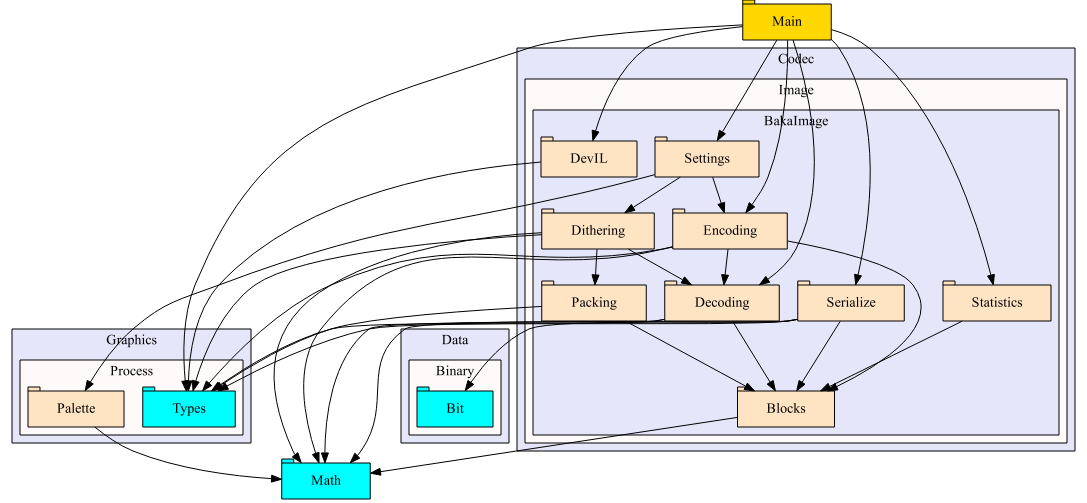
\includegraphics[width=0.8\textwidth]{img/structure}
  \caption{Структура модулей программы}
  \label{fig:structure}
\end{figure}

\subsection{Сжатие и распаковка}

Для хранения изображений внутри библиотеки используется библиотека
\texttt{repa}. Она предоставляет многомерные сжатые массивы для параллельных
расчётов. Расчёты на таких матрицах автоматически распараллеливаются, и
библиотека обеспечивает удобное API для работы с ними. Изображение параллельно
преобразовывается из его палитры в $YC_bC_r$, затем разбивается на блоки и
обрабатывается. Для сжатия на блоки и разворачивания блоков используются
оптимизированные функции, которые применяются по всей программе. Функции сжатия
принимают параметры, включая функции выбора палитры и распределения ошибки,
исходное изображение, и возвращают готовое представление формата в памяти.

Внутри функций сжатия большая часть вычислений производится в списках, так как
после компиляции большая часть из них преобразовывается из списков в
оптимизированные функции компилятором. Другая часть данных хранится в массивах,
предоставляемых библиотеками \texttt{repa} и \texttt{vector}. Поскольку массивы,
предоставляемые \texttt{repa}, откладывают собственные вычисления, в местах где
было очевидно что данные будут использоваться несколько раз запускался просчёт
массивов. Вся работа программы контроллировалась через функции измерения
относительной скорости работы функций и потребления памяти, предоставляемые
GHC. В итоге функции сжатия работают весьма оптимально, за счёт оптимизации
компилятором исключая множество лишних расчётов и при этом сохраняя краткость,
читаемость и красоту кода. Функции, которые работают с индексами (таких
меньшинство, в первую очередь, это две функции \texttt{blockify} и
\texttt{deblockifyBy} для работы с блоками) проверяются автоматически
генерируемыми тестами исходя из их свойств. Например, для функций собирания в
блоки и обратно, для любой данной матрицы и размера блоков будет верно что
преобразование туда и затем обратно должно быть равно исходной матрицы --
случайные тесты для этого генерируются языком автоматически, что даёт достаточно
высокую степень уверенности в отсутствии ошибок в программе.

Набор функций сжатия и распаковки написаны таким образом, что каскадно
используют друг друга. К примеру, функция \texttt{encodeChannel} параллельно
сжимает блоки с помощью функции \texttt{encodeBlock}, которой передаётся только
необходимая для сжатия блока информация. Функции распаковки дополнительно
позволяют получить плоское изображение, распакованное из блоков, но без замены
индексов на значения из палитр. Это используется для изменения частей
изображения без перепаковки.

Важное исключение из линейных, не считая обходов, функций сжатия составляет
функция подбора оптимального режима сжатия, которая пробует для каждого блока
несколько режимов в примерном порядке их качества, находя приемлемый по степени
ошибки.

Распаковка изображений, как и упаковка, производится параллельно сразу на этапе
преобразования цветов -- Haskell позволяет объединить все операции в одну без
каких-либо промежуточных массивов.

\subsection{Сохранение в файл и загрузка}

Для сохранения в файл и загрузки и работы с битами были написаны специальные
монады \texttt{GetBit} и \texttt{PutBit}, работающие поверх библиотеки Haskell
\texttt{binary}. Монады обеспечивают удобную работу с чтением и записью
отдельных групп бит, и производительны за счёт реализации в виде хвостовой
рекурсивной функции. Такие функции автоматически оптимизируются компилятором
языка в циклы, и при этом позволяют удобнее мыслить об алгоритме. Для этих монад
было найдено большое количество инвариантов, т.к. логика внутри достаточно
сложна, содержит много битовой арифметики и крайне предрасположена к ошибкам,
которые не обнаруживаются системой типов Haskell.

\subsection{Настройки сжатия}

В программе можно задавать настройки для всех отдельных каналов, задавать
произвольное количество режимов сжатия, размеров блоков и пикселей, уровни
допустимых ошибок и используемые алгоритмы. Пример конфигурационного файла
программы представлен в листинге~\ref{lst:conf}, однако предполагается, что по
результатам исследований будет найдена наиболее универсальная конфигурация
алгоритмов и режимов кодирования, так что единственной доступной пользователю
настройкой останется допустимый уровень ошибки. В целях исследования в
программе, тем не менее, оставлен полный функционал по настройке сжатия.

\begin{lstlisting}[float=p,caption={Пример конфигурации},label=lst:conf]
lumaChannel = [ BlockInfo { levels = 2
                          , sbsize = R.ix2 12 12
                          , pixel = R.ix2 2 2
                          , bitrate = 8
                          }
              , BlockInfo { levels = 4
                          , sbsize = R.ix2 12 12
                          , pixel = R.ix2 2 2
                          , bitrate = 8
                          }
              , BlockInfo { levels = 4
                          , sbsize = R.ix2 6 6
                          , pixel = R.ix2 1 1
                          , bitrate = 8
                          }
              , BlockInfo { levels = 2
                          , sbsize = R.ix2 3 3
                          , pixel = R.ix2 1 1
                          , bitrate = 8
                          }
              ]

colorChannel = [ BlockInfo { levels = 2
                           , sbsize = R.ix2 12 12
                           , pixel = R.ix2 2 2
                           , bitrate = 6
                           }
               , BlockInfo { levels = 4
                           , sbsize = R.ix2 12 12
                           , pixel = R.ix2 2 2
                           , bitrate = 6
                           }
               , BlockInfo { levels = 4
                           , sbsize = R.ix2 6 6
                           , pixel = R.ix2 1 1
                           , bitrate = 6
                           }
               , BlockInfo { levels = 2
                           , sbsize = R.ix2 3 3
                           , pixel = R.ix2 1 1
                           , bitrate = 6
                           }
               ]
               
lumaEncoding = EncodingInfo { palette = palette2
                            , dither = noDither
                            , threshold = 20
                            , errorK = 1.2
                            }
               
colorEncoding = EncodingInfo { palette = palette2
                             , dither = noDither
                             , threshold = 30
                             , errorK = 1.4
                             }

standardSettings = [ (Y, (lumaEncoding, lumaChannel))
                   , (Cb, (colorEncoding, colorChannel))
                   , (Cr, (colorEncoding, colorChannel))
                   ]
\end{lstlisting}

\subsection{Другие функции библиотеки}

Библиотека содержит в себе API для изменения уже сжатого изображения в пределах
установленных палитр. Это позволяет модифицировать изображения без потерь сжатия
в достаточно больших границах. Даже при необходимости пересчитывать новые
значения палитр это может быть сделано лишь в изменённых блоках, минимизируя
потери данных.

\subsection{Вывод}

Была написана обширная библиотека работы с предложенным нами форматом,
позволяющая выполнять все описанные выше операции работы с данным форматом и
дающая платформу для исследования оптимальных алгоритмов приведения изображения
в заданный формат.

\section{Исследовательский раздел}

\subsection{Введение}

В данном разделе нами описывается исследования и алгоритмы, используемые в
сжатии изображений в наш формат. Также демонстрируются результаты сжатия для
разных изображений.

\subsection{Метрика ошибки сжатия}

Для определения оптимального сжатия блоков второго уровня используется
предложенная нами метрика ошибки кодирования. Предположим, нам даны два
изображения (представленные в виде матриц) $A$ и $B$. Наша задача -- получить
число $e$, достоверно описывающую степень отклонения изображений друг от
друга. Суть алгоритма в следующем:

Вычтем изображения друг из друга. Для определённости пусть $C = A - B$. Разобьём
матрицу $C$ на матрицы размером 3х3 или меньше (на границах изображений). В
дальнейшем будем рассматривать эти матрицы по одной.

Наша задача -- для каждой такой матрицы найти наибольший связанный участок, все
элементы которого имеют один знак. Такая область называется ``серией''. Мы
выбираем области одного знака, поскольку такая область хорошо отражает
однородный пространственный всплеск ошибки в изображении. Обычно это
труднорешаемая задача, требующая аналогов алгоритмов на графах для поиска
максимального связанного подграфа. Однако, для блоков 3х3 есть две особенности,
позволяющие сильно ускорить этот процесс.

Все точки блока 3х3 лежат рядом с центральной точкой блока, так что взяв серию,
состояющую из центральной точки блока и других его точек одного с ней знака,
можно быстро получить, вероятно, достаточно большую серию. Исключение составляет
случай, когда центральная точка в матрице равна нулю -- тогда любая ненулевая
точка кроме неё может считаться с ней в одной серии, так что для нахождения
серии достаточно найти первую такую точку.

После нахождения серии мы действуем по одному из двух способов:

\begin{itemize}
\item Находим сумму квадратов точек серии: $$\sum x^2$$;
\item Находим сумму модулей точек серии: $$\sum |x|$$
\end{itemize}

Полученное число назовём $s$. В итоге искомой метрикой для блока будет число:
\[ e = \frac{s}{N} \]
, где $N$ -- количество точек в серии, а общей метрикой -- конечная
последовательность $e_i$ для всех блоков.

Эту метрику мы применяем следующим образом. Сначала для нашего лучшего варианта
сжатия мы считаем изменённую метрику $e_{bi}$:
\[ e_{bi} = k \cdot min(e_i, t) \]
, где $k$ -- коеффициент допустимости ошибок, а $t > 0$ -- отсекающий
фактор. Далее будет пояснена его необходимость.

Далее мы будем считать ошибку сжатия для каждого из проверяемых уровней сжатия,
начиная с наихудшего. Пусть последовательность ошибок для очередного уровня --
$e_{ti}$. Длины последовательностей $e_{ti}$ и $e_{bi}$ совпадают, сравним
попарно соответствующие ошибки. Если хоть одна ошибка из $e_{ti}$ меньше чем
текущая, текущий уровень сжатия отбрасывается и проверяется следующий.

Таким образом, коеффициент $k$ контроллирует допустимую расходимость ошибок
между лучшим вариантом сжатия и текущим. отсекающий фактор $t$ необходим в
случае, если какие-либо блоки целиком описываются заданными палитрами (ошибка
равна нулю). В таком случае один такой блок отбраковывает все уровни сжатия,
которые неидеально сохраняют это состояние. Фактор $t$, который выбирается
достаточно небольшим, препятствует такому раскладу.

Данная метрика позволяет с достаточно хорошими результатами выбирать подходящие
уровни сжатия. Использование разных способов нахождения $s$ даёт разные
результаты. Так, сумма квадратов сильнее выделяет резкие пики. Пример сравнения
статистики блоков для двух вариантов $s$ представлен в
таблице~\ref{tab:metric}. Схема алгоритма выбора оптимального уровня сжатия
блока представлена на рисунке~\ref{fig:blockopt}.

\begin{table}[h]
  \centering
  \begin{tabu} {|l|l|l|}
    Уровень & $x^2$ & $|x|$ \\
    \hline
    1 & 18\% & 20\% \\
    2 & 8\% & 12\% \\
    3 & 12\% & 14\% \\
    4 & 62\% & 54\% \\
  \end{tabu}
  \caption{Статистика для разных вариантов $s$}
  \label{tab:metric}
\end{table}

\begin{figure}
  \includegraphics[width=0.9\textwidth]{img/blockopt}
  \caption{Схема алгоритма выбора оптимального сжатия}
  \label{fig:blockopt}
\end{figure}

\subsection{Выбор палитры}

Для выбора палитры в целом, как уже было сказано выше, подходят любые алгоритмы
кластеризации. Размер палитры определяется исходя из заданных возможных уровней
сжатия с помощью алгоритмов, представленных выше. Однако когда размер уже
известен, необходимо выбрать точки палитры так, чтобы предложенная нами метрика
ошибки была минимальной.

Рассматривались несколько алгоритмов, которые будут описаны ниже.

\subsubsection*{Выбор средних}

Последовательность делилась по средней точке на две части рекурсивно, и от
каждой части искалась часть палитры. Так последовательность делится пока на
очередном шаге необходимая длина палитры не будет длины 1 -- тогда в качестве
палитры берётся средняя точка.

\subsubsection*{K-means}

Начальная палитра выбирается любым другим методом. Затем полученная палитра
уточняется с помощью алгоритма ближайших соседей.

\subsubsection*{2-палитра}

Рекурсия вглубь проходит так же, как в методе выбора средних. Однако здесь
есть дополнительная основа рекурсии на длине палитры 2, когда в качестве палитры
берутся крайние точки последовательности по значению.

\subsubsection*{Сравнение}

Статистика уровней сжатия для всех трёх методов выбора палитры показана в
таблице~\ref{tab:palette}. Из визуального сравнения видно, что метод K-means
позволяет резко улучшить качество изображения при использовании только двух
уровней для наименьших блоков размером 3х3.

\begin{table}[h]
  \centering
  \begin{tabu} {|l|l|l|l|}
    Уровень & Средние & K-means & 2-палитра \\
    \hline
    1 & 11\% & 11\$ & 4\% \\
    2 & 12\% & 16\% & 24\% \\
    3 & 45\% & 45\% & 23\% \\
    4 & 32\% & 28\% & 49\% \\
  \end{tabu}
  \caption{Статистика для разных алгоритмов выбора палитры}
  \label{tab:palette}
\end{table}

\subsection{Распределение ошибки}

Возможным этапом постобработки изображения является ``сглаживание'' ошибок
определения палитры (dithering). Это семейство алгоритмов, которые используют
особенность человеческого зрения меньше замечать случайные отклонения чем
постоянные искажения для улучшения изображения, сжатого с определённой палитрой.

Мы используем разновидность таких алгоритмов, называемую ``рапределением
ошибок'' (error diffusion). Известной разновидностью таких алгоритмов является,
например, алгоритм Флойда-Штейнберга~\cite{wiki:floyd}. Мы используем
модификацию этого алгоритма, описанную в~\cite{leptonica:colorquant}.
Общая идея алгоритма сводится к прохождению изображения слева направо, сверху
вниз и вычисления разницы между интенсивностью исходного изображения и сжатого в
данной точке. Эта ошибка передаётся с различными коеффициентами на окружающие
точки. В применении к предложенному формату необходима специальная модификация
алгоритма, работающая с различными палитрами в разных областях изображения.
Коеффициенты распостранения, используемые в нашей реализации, приведены на
рисунке~\ref{fig:dithermtx}.

Обработка изображения этим алгоритмом занимает относительно много
времени. Результат не отличается по степени сжатия (используется API для
модификации изображения без разсжатия), однако обладает чуть лучшими визуальными
свойствами.

\begin{figure}
  \centering
  \[
  \begin{bmatrix}
    0 & 0 & 0 \\
    0 & * & \frac{3}{8} \\
    0 & \frac{3}{8} & \frac{1}{4} \\
  \end{bmatrix}
  \]
  
  \caption{Коеффициенты для распределения ошибок}
  \label{fig:dithermtx}
\end{figure}

\subsection{Выбор уровней сжатия}

Как описано выше, формат предполагает произвольное количество произвольных
уровней сжатия. Нахождение оптимальных уровней аналитическим путём сводится к
нахождению оптимального значения многомерной функции. Однако, по времени работы
такое нахождение неприемлемо -- к тому же функция нелинейна и результат будет
оптимален лишь для одного конкретного изображения. Однако, на основе некоторых
эмпирических наблюдений и измерений можно построить набор оптимальных уровней
сжатия, дающих хороший баланс качества и сжатия.

Для начала определим, какими свойствами должен обладать хороший набор настроек
сжатия:
\begin{itemize}
\item Он должен использоваться (процент его использования в изображениях в
  средним относительно качества его сжатия и положения среди уровней должен быть приемлем);
\item Наиболее сильный уровень сжатия должен давать приемлемые по качеству
  результаты, если всё изображение будет сжато исключительно им;
\item Наиболее слабый уровень должен обладать размером, способствующим
  равномерному выбору уровней сжатия;
\item Количество уровней сжатия должно быть степенью двойки.
\end{itemize}

Поясним эти требования. Первое требование разумно само по себе, поскольку если
уровень не используется в изображениях, он зря занимает место среди
остальных. Второе условие исходит из того, что лучший получаемый уровень
качества для данного набора уровней -- это изображение, целиком сжатое с помощью
последнего уровля. Третье условие получается из того, что индекс уровня
кодируется в блоках в двоичной системе счисления, и чтобы полностью заполнить
область значений индекса, разумно иметь кратное количество уровней.

Блок 3х3 является, из-за особенностей нашей метрики, удобным для
использования. Будем исходить из такого размера как минимального размера
блока. Как мы выяснили из визуального эксперимента, блоки 3х3 с двумя уровнями
являются оптимальными с точки зрения размер/качество при оптимальном выборе
палитры для фотографических и сканированных изображений. Возьмём их за минимум.

При повышении максимального размера блока в два раза наблюдается резкий скачок
во время перехода с размера блока 12х12 на 24х24, в котором (для фотографических
изображений) качество сжатия сильно ухудшается из-за слишком большой области
обхвата, в которой блоки должны быть сжаты одинаковым уровнем сжатия. Таким
образом, оптимальным максимальным размером блока было решено выбрать 12х12.

После этого мы изучили различные конфигурации из четырёх уровней сжатия с
крайними -- сжатием на два уровня по блокам 12х12 и 3х3. Выяснилось, что блок
6х6 с двумя уровнями используется слишком мало. Таким образом, в качестве
средних были выбраны блоки 12х12 и 6х6 с четырьмя уровнями. Этот набор
обеспечивает стабильное распределение использований уровней с креном в сторону
слабого сжатия, что соответствует распределению деталей на изображении.

\subsection{Вывод}
Мы исследовали возможные алгоритмы, применяемые в сжатии и отобрали оптимальные
для использования в стандартных настройках сжатия. Мы также нашли метрику,
хорошо описывающую ошибку сжатия изображения, и способ нахождения оптимальной
степени сжатия при помощи этой метрики. Наконец, мы нашли оптимальную
конфигурацию уровней сжатия, обеспечивающую хороший компромисс между сжатием и
качеством и равномерно используемую в среднем по различным изображениям.

\section{Организационно-экономический раздел}
\subsection{Введение}
В данной части производится расчёт и обоснование стоимости производства разработанного программного комплекса, выполняющего поставленную задачу.
Исходя из анализа существующих на рынке коммерческих решений, можно сделать вывод о приблизительной стоимости готового ПП --- в среднем цена составляет 30~000 руб за одну бессрочную лицензию.

\subsection{Организация и планирование процесса разработки}
При использовании традиционного подхода, организация и планирование процесса разработки программного продукта или программного комплекса предусматривает выполнение следующих работ:

\begin{itemize}
\item формирование состава выполняемых работ и группировка их по стадиям разработки;
\item расчет трудоемкости выполнения работ;
\item установление профессионального состава и расчет количества исполнителей;
\item определение продолжительности выполнения отдельных этапов разработки;
\item построение календарного графика выполнения разработки;
\end{itemize}

Планирование длительности этапов и содержания проекта осуществляется в соответствии с ЕСПД ГОСТ 34.603-92 и распределяет работы по этапам, как показано в таб.~\ref{tab:econ-stages}

\begin{table}[H]
  \begin{tabu}{|c|c|X[l]|}\hline
    Основные стадии & № & Содержание работы \\\hline
    \multirow{2}{*}{Техническое задание} & 1 & Постановка задачи \\\cline{2-3}
         & 2 & Выбор средств разработки и реализации \\\hline
    \multirow{2}{*}{Эскизный проект} & 3 & Разработка математической модели \\\cline{2-3}
         & 4 & Разработка алгоритмов расчёта задачи \\\hline     
    \multirow{2}{*}{Техно-рабочий проект} & 5 & Реализация алгоритмов расчёта задачи \\\cline{2-3}
         & 6 & Разработка пользовательского интерфейса \\\cline{2-3}            
         & 7 & Реализация пользовательского интерфейса \\\hline
    Внедрение & 8 & Проведение вычислительных экспериментов \\\hline
  \end{tabu}
  \caption{Распределение работ по этапам.}
  \label{tab:econ-stages}
\end{table}

\subsection{Расчёт трудоёмкости выполнения работ}
Трудоемкость разработки программной продукции зависит от ряда
факторов, основными из которых являются следующие:
\begin{itemize}
  \item степень новизны разрабатываемого программного комплекса,
  \item сложность алгоритма его функционирования,
  \item объем используемой информации, вид ее представления и способ обработки,
  \item уровень используемого алгоритмического языка программирования
\end{itemize}

Исходные данные расчета приведены в табл.~\ref{tab:econ-init}.

\begin{table}[H]
  \begin{tabu}{|X[l]|>{\centering}m{1.5cm}|X[l]|}\hline
    Функциональное назначение ПП & & Задачи расчётного характера \\\hline
    Алгоритм разработки ПП & 2в &  \\\hline
    Группа новизны & В & Разработка программной продукции, имеющей аналоги \\\hline
    Степень сложности & 1-я группа & Программная продукция, реализующая оптимизационные и моделирующие алгоритмы \\\hline
	По виду представления исходной информации & Группа 12 & Форматный контроль информации. \\\hline
  \end{tabu}
  \caption{Исходные данные}
  \label{tab:econ-init}
\end{table}

Трудоемкость разработки программной продукции $\tau_{ПП}$ может быть определена как сумма величин трудоемкости выполнения отдельных стадий разработки ПП из выражения:

\begin{equation}
	\tau_{ПП} = \tau_{ТЗ} + \tau_{ЭП} + \tau_{ТП} + \tau_{HG} + \tau_{В} 
\end{equation}

где 
\begin{itemize}
  \item $\tau_{ТЗ}$ - трудоемкость разработки технического задания на создание ПП;
  \item $\tau_{ЭП}$ - трудоемкость разработки эскизного проекта ПП;
  \item $\tau_{ТП}$ - трудоемкость разработки технического проекта ПП;
  \item $\tau_{HG}$ - трудоемкость разработки рабочего проекта ПП;
  \item $\tau_{В}$ - трудоемкость внедрения разработанного ПП.
\end{itemize}

Трудоемкость разработки технического задания рассчитывается по формуле:
\begin{equation}
	\tau_{ТЗ} = Т_{ЗРЗ} + Т_{ЗРП}
\end{equation}
где 
\begin{itemize}
  \item $Т_{ЗРЗ}$ - затраты времени разработчика постановки задач на разработку ТЗ, чел. дни;
  \item $Т_{ЗРП}$ - затраты времени разработчика программного обеспечения на разработку ТЗ, чел. дни.
\end{itemize}

В расчёте участвуют следующие коэффициенты:
\begin{itemize}
  \item $t_З = 20$ – норма времени на разработку ТЗ на программный продукт в зависимости от функционального назначения и степени новизны разрабатываемого ПП, чел. дни;
  \item $K_{ЗРЗ} = 0.65$ - коэффициент, учитывающий удельный вес трудоемкости работ, выполняемых разработчиком постановки на стадии ТЗ;
  \item $K_{ЗРП} = 0.35$ - коэффициент, учитывающий удельный вес трудоемкости работ, выполняемых разработчиком программного обеспечения на стадии ТЗ.
\end{itemize}

Тогда
\begin{equation}
	\tau_{ТЗ} = 20 (0.65 + 0.35) = 20 \text{ [чел. дни]}
\end{equation}

Аналогично рассчитывается трудоёмкость эскизного проекта ПП $\tau_{ЭП}$:
\begin{equation}
	\tau_{ЭП} = t_{ЭП} (К_{ЭРЗ} + К_{ЭРП}) = 20 (0.75 + 0.25) = 20 \text{ [чел. дни]}
\end{equation}

Трудоемкость разработки технического проекта $\tau_{ТП}$ зависит от функционального назначения ПП, количества разновидностей форм входной и выходной информации и определяется как сумма времени, затраченного разработчиком постановки задач и разработчиком программного обеспечения, т.е.
\begin{gather*}
	\tau_{ТП} = (t_{ТРЗ} + t_{ТРП}) К_В К_р \\
	К_В = (К_П n_П + К_{НС} n_{НС} + К_Б n_Б) / (n_П + n_{НС} + n_Б)
\end{gather*}

где 
\begin{itemize}
  \item $t_{ТРЗ} = 37, t_{ТРП} = 23$ - норма времени, затрачиваемого на разработку технического проекта разработчиком постановки задач и разработчиком ПП соответственно, чел.-дни
  \item $К_Р = 1,26$ - коэффициент учета режима обработки информации
  \item $К_П = 1, К_НС = 0,72, К_Б = 2.18$ - значения коэффициентов учета вида используемой информации для переменной, нормативно-справочной информации и баз данных соответственно
  \item $n_П = 6, n_НС = 4, n_Б = 0$ - значения коэффициентов учета вида используемой информации для переменной, нормативно-справочной информации и баз данных соответственно
\end{itemize}
Тогда 
\begin{gather*}
	\tau_{ТП} = (37 + 23) (1 \cdot 6 + 0.72 \cdot 4 + 2.18 \cdot 0) / (6 + 4 + 0) \cdot 1.26 = 67 \text{ [чел. дни]}
\end{gather*}

Трудоемкость разработки рабочего проекта $\tau_{РП}$ зависит от
функционального назначения ПП, количества разновидностей форм входной
и выходной информации, сложности алгоритма функционирования,
сложности контроля информации, степени использования готовых
программных модулей, уровня алгоритмического языка программирования и
определяется по формуле:
\begin{gather*}
  \tau_{РП} = К_к К_р К_Я К_З К_{ИА} (t_{РРЗ} + t_{РРП})\\
  К_{ИА} = (К_П' n_П + К_{НС}' n_{НС} + К_Б' n_Б) / (n_П + n_{НС} + n_Б)
\end{gather*}
где
\begin{itemize}
  \item $t_{РРЗ} = 102, t_{РРП} = 348$ - норма времени, затраченного на разработку РП на алгоритмическом языке высокого уровня разработчиком постановки задач и разработчиком программного обеспечения соответственно, чел. дни.
  \item $K_К = 1$ – коэффициент учета сложности контроля информации;
  \item $К_Р = 1.32$ - коэффициент учета режима обработки информации
  \item $K_Я = 1$ – коэффициент учета уровня используемого алгоритмического языка программирования;
  \item $K_З = 0.8$ – коэффициент учета степени использования готовых программных модулей;
  \item $K_{ИА}$ – коэффициент учета вида используемой информации и сложности алгоритма ПП;
  \item $К_П' = 1.20, К_НС' = 0.65, К_Б' = 0.54$ - значения коэффициентов учета сложности алгоритма ПП и вида используемой информации для переменной, нормативно-справочной информации и баз данных соответственно.
\end{itemize}
Тогда
\begin{gather*}
  К_{ИА} = 6 \cdot 1.20 + 4 \cdot 0.65 / (4 + 6) = 0.98 \\
  \tau_{РП} = 1 \cdot 1.32 \cdot 1 \cdot 0.8 \cdot 0.98 \cdot(102 + 348) = 466 \text{ [чел. дни]}
\end{gather*}

Так как при разработке ПП стадии «Технический проект» и «Рабочий
проект» объединены в стадию «Техно-рабочий проект», то трудоемкость ее
выполнения $\tau_{ТРП}$ определяется по формуле:
\begin{gather*}
  \tau_{ТРП} = 0.85 \tau_{ТП} + \tau_{РП} = 0.85 \cdot 67 + 466 = 523 \text{ [чел. дни]}
\end{gather*}

Трудоемкость выполнения стадии внедрения $\tau_{В}$ может быть рассчитана по формуле:
\begin{gather*}
  \tau_{В} = К_к К_р К_З (t_{ВРЗ} + t_{ВРП}) = 1 \cdot 1.32 \cdot 0.8 (30 + 68) = 103 \text{ [чел. дни]}
\end{gather*}

Трудоемкости по этапам разработки проекта представлены в таблице~\ref{tab:econ-trud}.

\begin{table}[H]
  \begin{tabu}{|X[c]|X[c]|}\hline
    Этап & Трудоёмкость этапа, [чел. дни] \\\hline  
    ТЗ & 20 \\\hline  
    ЭП & 20 \\\hline  
    ТРП & 533 \\\hline  
    В & 103 \\\hline      
    Итого & 676 \\\hline        
  \end{tabu}
  \caption{Трудоемкости по стадиям разработки проекта}
  \label{tab:econ-trud}
\end{table}

Средняя численность исполнителей при реализации проекта разработки и внедрения ПО определяется соотношением $N = \frac{Q_p}{F}$, 
где
\begin{itemize}
  \item $Q_p = \tau \cdot t_p$ - затраты труда на выполнение проекта (разработка и внедрение ПО),
  \item $F = T \cdot F_M$ - фонд рабочего времени;
  \item $Т$ - время выполнения проекта в месяцах. T = 5 мес.;
  \item $F_M$ - фонд времени в текущем месяце, который рассчитывается из учета общества числа дней в году, числа выходных и праздничных дней и определяется соотношением $F_М = \frac{t_p (D_k - D_B - D_П)}{12}$;
  \item $t_p$ - продолжительность рабочего дня;
  \item $D_K$ - общее число дней в году;
  \item $D_B$ - число выходных дней в году;
  \item $D_П$ - число праздничных дней в году.
\end{itemize}

Тогда 
\begin{gather*}
  F = 5 \cdot 8 (365 - 103 - 13) / 12 = 830\\
  N = 676 \cdot 8 / 830 = 7 \text{ - число исполнителей проекта.}
\end{gather*}

\subsection{Календарный план-график}
Планирование и контроль хода выполнения разработки проводится по календарному графику выполнения работ. Планирование процесса разработки и календарный ленточный план представлены в таб. \ref{tab:econ-plan} и рис. \ref{tab:econ-lent} соответственно.

\begin{table}[H]
  \begin{tabu} to \textwidth {|m{2cm}|m{1,5cm}|m{4cm}|m{3cm}|X|}\hline
    Стадия & $\tau$ & Должность исполнителя & Распределение трудоемкости & Числ-ть \\\hline
    ТЗ & 20 & \shortstack{Ведущий инженер\\Программист} & \shortstack{15(75 \%)\\5} & \shortstack{1\\1} \\\hline  
    ЭП & 20 & \shortstack{Ведущий инженер\\Программист} & \shortstack{12(60 \%)\\8} & \shortstack{1\\1} \\\hline  
    ТРП & 533 & \shortstack{Ведущий инженер\\Программист} & \shortstack{71\\6 \times 76} & \shortstack{1\\6} \\\hline  
    В & 103 & \shortstack{Ведущий инженер\\Программист} & \shortstack{13\\3 \times 30} & \shortstack{1\\3} \\\hline      
    Итого & 676 & & & 7 \\\hline  
  \end{tabu}
  \caption{Планирование процесса разработки.}
  \label{tab:econ-plan}
\end{table}

\begin{figure}[H]
  \centering
  \includegraphics[width=.5\textwidth]{img/timeplan}
  \caption{Календарный ленточный план работ.}
  \label{tab:econ-lent}
\end{figure}

Вывод: при распараллеливании работы ведущего инженера и
программистов можно добиться сокращения срока разработки и внедрения
программного продукта с 676 дней до 133 дней, т. е. в 5.08 раза по сравнению
со временем разработки одним человеком.

В таб. \ref{tab:econ-salary} приведены затраты на заработную плату и отчисления
на социальное страхование в пенсионный фонд, фонд занятости и фонд
обязательного медицинского страхования (30\%). Для всех исполнителей
предполагается оклад в размере 20000 рублей в месяц.

\begin{table}[H]
  \centering
  {
  \begin{tabu} to \textwidth {||c|*{3}{|X|X|X|}|c||}\hline
   & \multicolumn{3}{c||}{Г.И.} & \multicolumn{3}{c||}{П1} & \multicolumn{3}{c||}{П2..6} & Всего \\\hline
   Мес & Р.Д. & ЗП & ЕСН & Р.Д. & ЗП & ЕСН & Р.Д. & ЗП & ЕСН & \\\hline
   1 & 21 & 20 & 6 & 10 & 9.52 & 2.86 &  &  &  & 38.38 \\\hline
   2 & 21 & 20 & 6 & 11 & 10.48 & 3.14 & 7 & 6,67 & 2 & 48.29 \\\hline
   3 & 21 & 20 & 6 & 21 & 20 & 6 & 21 & 20 & 6 & 78.00 \\\hline
   4 & 21 & 20 & 6 & 21 & 20 & 6 & 21 & 20 & 6 & 78.00 \\\hline
   5 & 21 & 20 & 6 & 21 & 20 & 6 & 21 & 20 & 6 & 78.00 \\\hline
   6 & 20 & 19.05 & 5.71 & 21 & 20 & 6 & 21 & 20 & 6 & 76.76 \\\hline
   \multicolumn{10}{||l||}{Итого:}  & 320.67 \\\hline   
  \end{tabu}}
  \caption{Затраты на зарплату и отчисления на социальное страхование, тыс.руб.}
  \label{tab:econ-salary}
\end{table}

Расходы на материалы, необходимые для разработки программной
продукции, указаны в таблице \ref{tab:econ-materials}.

\begin{table}[H]
  \centering
  \begin{tabu} to \textwidth {|c|c|X|X|X|}\hline
    Наименование & Единица & К-во & Цена/ед. & Сумма \\
    материала & измерения & & (руб.)& (руб.) \\\hline
    Бумага А4 & Пачка 500 листов & 2 & 200 & 400\\\hline
    Картридж Canon IP5200 & Картридж, 10мл & 5 & 300 & 1500\\\hline
    \multicolumn{4}{|l|}{Итого:} & 1900 \\\hline
  \end{tabu}
  \caption{Затраты на материалы.}
  \label{tab:econ-materials}
\end{table}

В работе над проектом используется специальное оборудование –
персональные электронно-вычислительные машины (ПЭВМ) в количестве 14
шт. Стоимость одной ПЭВМ составляет 20~000 рублей. Согласно нормативным документам, срок амортизации ПЭВМ составляет 3 года, что определяет месячную норму амортизации K = 2.7\%.

Тогда за 5 месяцев работы расходы на амортизацию составят $20~000 \cdot 14 \cdot 0.027 \cdot 5 = 37~800 \text{руб.}$

Общие затраты на разработку ПП составят:

\begin{gather*}
  C = 320~670 + 1~900 + 37~800 = 360~370 \text{ руб.}
\end{gather*}

\subsection{Расчёт стоимости программного продукта}
Цена ПП рассчитывается по формуле:
\begin{gather*}
  Ц = С + Пр\\
  Пр = \frac{(С-С_м)р_н}{100 \%}
\end{gather*}
где
\begin{itemize}  
 \item $С$ - затраты на разработку ПП\\
 \item $С_м$ - материальные затраты, руб./изд\\
 \item $Пр$ - желаемая прибыль\\ 
 \item $р_н$ - норматив рентабельности, принимаемый разработчиком\\  
\end{itemize}

Тогда
\begin{gather*}
  Ц = 360~370 + (360~370 - 37~800 - 1~900) \cdot 0.25 = 440~538 \text{ руб.}
\end{gather*}

\subsection{Расчет экономической эффективности}

Основными показателями экономической эффективности является
чистый дисконтированный доход (ЧДД) и срок окупаемости вложенных
средств.

Чистый дисконтированный доход определяется по формуле:
\begin{gather*}
  ЧДД = sum_{t=0}^T (R_t - З_t) \frac{1}{(1 + E)^t}
\end{gather*}
где
\begin{itemize}
  \item $Т$ - горизонт расчета по месяцам;
  \item $t$ - период расчета;
  \item $R_t$ - доход за текущий месяц;
  \item $З_t$ - затраты за текущий месяц;
  \item $E$ - приемлемая для инвестора норма прибыли на вложенный капитал.
\end{itemize}

Коэффициент E установим равным ставке рефинансирования ЦБ РФ – 8.25\%
годовых (или 0.66\% в месяц). В виду особенности разрабатываемого продукта
он может быть продан лишь однократно.
Коэффициент дисконтирования равен 1/(1 + Е) = 0.99.

В таб. \ref{tab:econ-chdd} приведен расчет ЧДД по месяцам работы над проектом.

График ЧДД приведён на рис.~\ref{fig:econ-chdd}.
\begin{table}[H]
  \centering
  \begin{tabu} to \textwidth {|c|X|X|X|X|}\hline
    Месяц & Тек. Затр. & Общ. Затр. & Тек.доход & ЧДД \\\hline
    1 & 46130,95 & 46130,95 & 0,00 & -45669,64 \\\hline
    2 & 56035,71 & 102166,67 & 0,00 & -84815,30 \\\hline
    3 & 85750,00 & 187916,67 & 0,00 & -142790,67 \\\hline
    4 & 85750,00 & 273666,67 & 0,00 & -208511,45 \\\hline
    5 & 85750,00 & 359416,67 & 0,00 & -314784,59 \\\hline
    6 & 84511,90 & 443928,57 & 440538,00 & 20406,92 \\\hline
  \end{tabu}
  \label{tab:econ-chdd}
  \caption{Расчёт ЧДД.}
\end{table}

\begin{figure}[H]
  \centering
  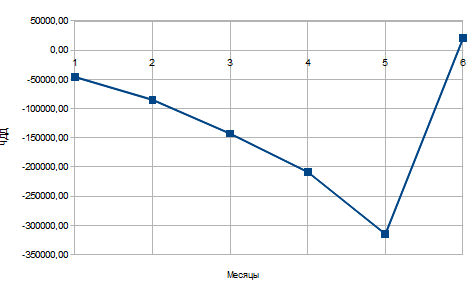
\includegraphics[width=.9\textwidth]{img/chddplot}
  \caption{График изменения чистого дисконтированного дохода.}
  \label{fig:econ-chdd}
\end{figure}

\subsection{Вывод}
Исходя из расчётов, можно сделать вывод о том, что проект окажется рентабельным, а затраты на его выполнение
окупятся. Итоковый ЧДД равен 20~406.92 рублей. Срок реализации проекта составляет 6 месяцев.
\section{Охрана труда}
\subsection{Введение}

В процессе создания ПО эксплуатирующий его персонал подвергается воздействию ряда опасных и вредных факторов, среди которых можно перечислить электромагнитное излучение, отражённый свет, блики и шум.

В данном разделе рассматриваются основные виды опасных и вредных факторов, и на основе их анализа вырабатываются требования к рабочему помещению на основе требований СанПиН.

\subsection{Анализ опасных и вредных факторов}
\subsubsection{Микроклимат}

Работа программиста относится к категории 1а (не предполагает физических усилий). Поэтому нормы микроклимата определяются таблицей ~\ref{table:climate}.

\begin{table}[h]
  \begin{tabu}{|X[c]|X[c]|X[c]|X[c]|}\hline
    & \shortstack{Температура\\воздуха, $^\circ \mathrm{C}$} 
    & \shortstack{Отн. влажность\\воздуха, \%}
    & \shortstack{Скорость движ.\\воздуха, м/с}\\\hline 
    Холодный & 22-24 & 40-60 & 0,1 \\\hline
    Теплый & 23-25 & 40-60 & 0,1 \\\hline
  \end{tabu}
  \caption{Оптимальные нормы микроклимата}
  \label{table:climate}
\end{table}

Для борьбы с запылённостью помещения, являющейся ещё более вредным фактором в сочетании с электростатическими полями ПК, предусмотрено использование системы кондиционирования. Использование подобной системы также позволяет регулировать показатели температуры, влажности и скорости движения воздуха. 

Нормы СанПиН 2.2.4.1294-03 определяют уровни содержания ионов
в воздухе (таблица ~\ref{table:ions}). Для обеспечения требуемых уровней предусмотрено использование системы ионизации воздуха.

\begin{table}[h]
  \begin{tabu}{|X[c]|X[c]|X[c]|}  
    \hline
    \multirow{2}{*}{Уровни} & \multicolumn{2}{|c|}{Число ионов в 1 см куб. воздуха} \\\cline{2-3}
    & $n^+$ & $n^-$\\\hline
    Минимально необходимые & 400 & 600 \\\hline
    Оптимальные & 1500-3000 & 3000-5000 \\\hline
    Предельно допустимые & 50000 & 50000 \\\hline
  \end{tabu}
  \caption{Уровни ионизации воздуха помещений при работе на ПЭВМ}
  \label{table:ions}
\end{table}


\subsubsection{Шум}

При разработке программного обеспечения внутренними источниками шума являются вентиляторы, а также принтеры и другие периферийные устройства ЭВМ. Внешние источники шума – прежде всего, шум с улицы и из соседних помещений. Постоянные внешние источники шума, превышающего нормы, отсутствуют. План помещения с источниками света дан на рисунке ~\ref{fig:srvplan}. Габариты помещения даны в таблице ~\ref{table:srvsize}. Вспомогательные расчётные параметры даны в таблице ~\ref{table:srvparams}. Характеристики источников шума (положение, расстояние, уровни звуковой мощности и расчётная площадь) и спектральные параметры помещения даны в таблице ~\ref{table:srvnoisesrc}. Расчётные и предельные уровни звуковой интенсивности для напольных источников шума даны в таблице ~\ref{table:srvnoiseint}. Расчётный и предельный спектры даны на рисунке ~\ref{fig:srvspectrum}.

Как видно из расчётов, расчётный спектр превышает предельно допустимый уровень шума. Определено, что увеличение Ri - расстояния до источников шума
слабо влияет на уровень шума. Изменение габаритов комнаты, однако, может в значительной мере повлиять на уровень шума в помещении в
целом, но по результатам расчётов также не позволяет снизить его до допустимых значений. Действенным защитным мероприятием в этом
Случае будет являться введение звукоизоляции, акустическая обработка помещения. Также возможно вынесение рабочих мест за пределы зашумлённого помещения, где, в случае оборудования данного помещения звукопоглощающими покрытиями (прорезиненные ковры, пористые покрытия, ширмы, многослойные покрытия с воздушным промежутком), уровни звукового давления будут допустимыми.

\begin{figure}[h]
  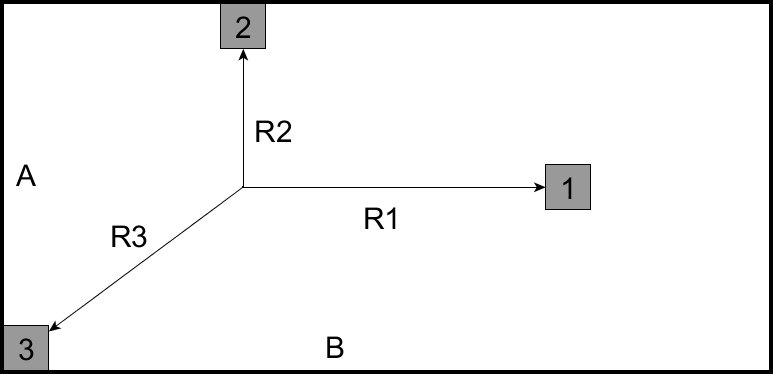
\includegraphics[width=\textwidth]{img/srvplan.png}
  \caption{Схема расположения расчётной точки относительно источников шума}
  \label{fig:srvplan} 
\end{figure}

\begin{table}[h]
\centering
\begin{minipage}[t]{.45\textwidth}
  \centering
  \begin{tabu}{|X[c]|X[c]|}\hline
    Длина(А) & 15 \\\hline
    Ширина(В) & 30 \\\hline
    Высота(С) & 4 \\\hline
    Объем(V) & 1800 \\\hline
  \end{tabu}
  \caption{Габариты комнаты}
  \label{table:srvsize}
\end{minipage}
\hfil
\begin{minipage}[t]{.45\textwidth}
  \centering
  \begin{tabu}{|X[c]|X[c]|}\hline
    Ф & 1 \\\hline
    Х & 1 \\\hline
    B1000 & 90 \\\hline
    æ & 1 \\\hline
  \end{tabu}
  \caption{Вспомогательные пар-ры}
  \label{table:srvparams}
\end{minipage}
\end{table}

\begin{table}[h]
  \begin{tabu}{|c|c|c|c|c|c|c|c|c|c|c|X[c]|}
    \hline
    \multirow{2}{*}{№} &
    \multirow{2}{*}{\shortstack{Тип\\монтажа}} &    
    \multirow{2}{*}{$R_i$} & 
    \multicolumn{8}{|c|}{Ур-нь звуковой мощности, Lw для окт. полос} &
    \multirow{2}{*}{S} \\\cline{4-11}      
     & & & 63 & 125 & 250 & 500 & 1000 & 2000 & 4000 & 8000 & \\\hline
    1 & подвешен & 9 & 81 & 82 & 83 & 84 & 83 & 81 & 80 & 77 & 508 \\\hline
    2 & на полу & 9 & 90 & 91 & 98 & 99 & 97 & 93 & 91 & 86 & 254 \\\hline
    3 & на полу & 9 & 84 & 82 & 84 & 91 & 94 & 94 & 91 & 91 & 127 \\\hline 
    
    \multicolumn{2}{c}{} & \multicolumn{9}{|c|}{Спектральные параметры помещения} & \multicolumn{1}{c}{}\\\cline{3-11}
    \multicolumn{2}{c|}{} & y & 0,5 & 0,5 & 0,55 & 0,7 & 1 & 1,6 & 3 & 6\\\cline{3-11}
    \multicolumn{2}{c|}{} & B & 45 & 45 & 49,5 & 63 & 90 & 144 & 270 & 540\\\cline{3-11}
  \end{tabu}
  \caption{Параметры источников звука и спектральные параметры помещения}
  \label{table:srvnoisesrc}
\end{table}

\begin{table}[h]
  \begin{tabu}{|X[c]|X[c]|X[c]|X[c]|X[c]|X[c]|X[c]|X[c]|X[c]||}
    \hline
    № &
    \multicolumn{8}{|c|}{Уровни звуковой интенсивности, Lj}\\\hline
    2 & 79,68 & 80,68 & 87,28 & 87,29 & 83,85 & 78,01 & 73,73 & 66,55 \\\hline
    3 & 73,86 & 71,86 & 73,48 & 79,53 & 81,19 & 79,52 & 74,56 & 72,84 \\\hline
    $Lj_{sum}$ & 80,69 & 81,21 & 87,46 & 87,96 & 85,73 & 81,84 & 77,17 & 73,75 \\\hline
    $L_{lim}$ & 83 & 74 & 68 & 63 & 60 & 57 & 55 & 54 \\\hline
  \end{tabu}
  \caption{Расчётные и предельные уровни звуковой интенсивности}
  \label{table:srvnoiseint}
\end{table}

\begin{figure}[h]
  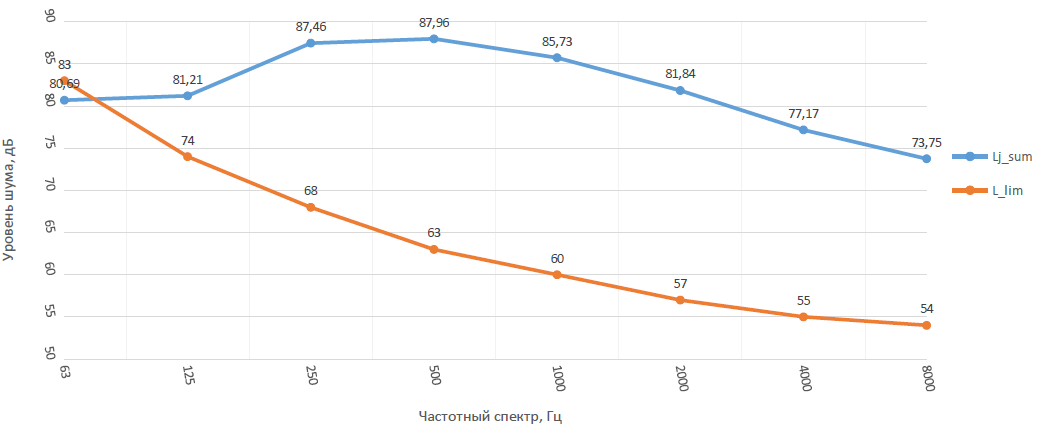
\includegraphics[width=\textwidth]{img/spectrum.png}
  \caption{Расчётный и предельный спектры}
  \label{fig:srvspectrum}
\end{figure}

\subsubsection{Электробезопасность}

При работе с ПК работник подвергается повышенному риску удара электрическим током, поскольку проводит много времени около корпуса компьютера. Для работы за компьютером он должен быть оборудован защитным заземлением в соответствии с техническими требованиями.

\subsubsection{Свет}

Одним из основных опасных и вредных факторов при работе за компьютером является повышенная нагрузка на глаза. Отсюда следующие общие требования:
\begin{itemize}
	\item Окна должны быть ориентированы преимущественно на север и северо-восток
	\item Коэффициенты отражения должны составлять 0,7-0,8 для потолка, 0,5-0,6 для стен и 0,3-0,5 для пола.
	\item Окна должны быть оборудованы средствами регулирования (жалюзи, занавеси)
\end{itemize}

Требования к освещению на рабочих местах представлены в таблице ~\ref{table:lightreq}.
\begin{table}[h]
  \begin{tabu}{|X[c]|X[c]|}\hline
    Освещенность на поверхности стола & 300 - 500 лк. \\\hline
    Освещенность поверхности экрана & <300 лк. \\\hline
    \shortstack{Яркость светящихся поверхностей\\(окна, светильники и др.),\\ находящихся в поле зрения} & 200 кд/м2. \\\hline
    Показатель ослепленности & <20 \\\hline
    Яркость светильников общего освещения & <200 кд/м2 \\\hline
    Коэффициент запаса (Кз) & 1.4 \\\hline
    Коэффициент пульсации & 5\% \\\hline
  \end{tabu}
  \caption{Требования к освещению на рабочих местах с ПК}
  \label{table:lightreq}
\end{table}

Расчёт освещения в соответствии с планом помещения был произведён в программе DIALux 4.12.01. План помещения и ведомость объектов даны на рисунке ~\ref{fig:lightplan} и таблице ~\ref{table:lightitemlist} соответственно. Паспорт светильника предоставлен на рисунке ~\ref{fig:lightpassport}. Данные светотехнических результатов расчёта даны на рисунке ~\ref{fig:lighttechres}. План помещения с указанием изолиний освещённости и ведомость светильников даны на рисунке ~\ref{fig:lightiso}. 3D-визуализация помещения дана на рисунке ~\ref{fig:light3d}.

\begin{figure}[h]
  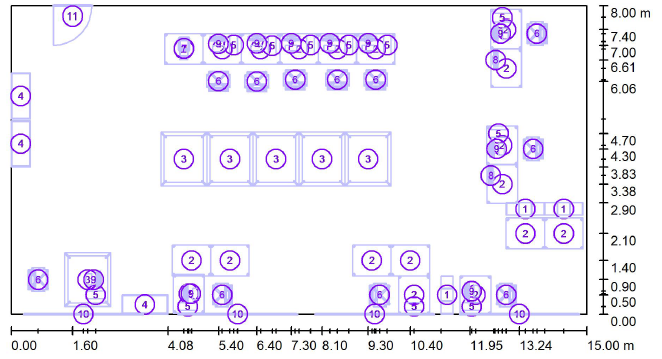
\includegraphics[width=\textwidth]{img/lightplan}
  \caption{План помещения}
  \label{fig:lightplan}
\end{figure}

\begin{table}[h]
  \begin{tabu}{|X[c]|X[c]|X[c]|}\hline
    № & Шт. & Обозначение \\\hline
    1 & 3 & 100x200 квадрат \\\hline
    2 & 19 & 100x80 стандарт. \\\hline
    3 & 6 & 120x140 дельта \\\hline
    4 & 3 & 120x200 2двери \\\hline
    5 & 11 & компьютер t \\\hline
    6 & 11 & офисный стул 1 \\\hline
    7 & 1 & принтер t \\\hline
    8 & 2 & экран TFT \\\hline
    9 & 10 & экран TFT и клавиатура \\\hline
    10 & 4 & Окно \\\hline
    11 & 1 & Дверь \\\hline
  \end{tabu} 
  \caption{Ведомость объектов}
  \label{table:lightitemlist}
\end{table}

\begin{figure}[h]
  \centering
  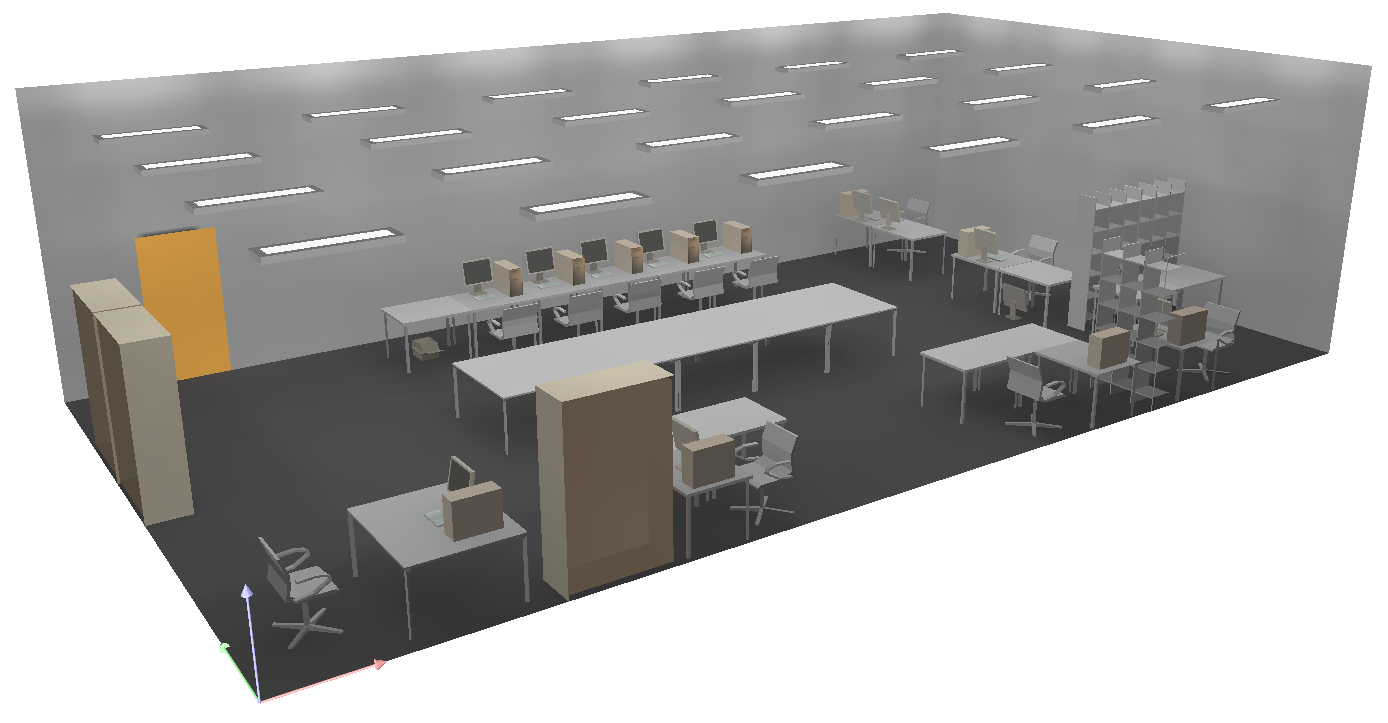
\includegraphics[width=\textwidth]{img/light3d}
  \caption{3D-визуализация помещения}
  \label{fig:light3d}
\end{figure}

\clearpage
\begin{figure}[h]
  \centering
  \includegraphics[page=3,height=.8\textheight]{img/lightcalc}
  \caption{Паспорт светильника}
  \label{fig:lightpassport}
\end{figure}

\clearpage
\begin{figure}[h]
  \centering
  \includegraphics[page=8,height=.8\textheight]{img/lightcalc}
  \caption{Светотехнические результаты}
  \label{fig:lighttechres}
\end{figure}

\clearpage
\begin{figure}[h]
  \centering
  \includegraphics[page=4,height=.8\textheight]{img/lightcalc}
  \caption{Резюме светового расчёта}
  \label{fig:lightiso}
\end{figure}
\clearpage

\subsection{Вывод}

В результате анализа санитарных норм в соответствии с ними в данном разделе были выработаны требования к рабочему помещению. На основании данных требований был спланирован интерьер помещения с указанием расположения светоизлучающих элементов. Спланированное помещение соответствует условиям по безопасности помещений и охране труда.

Был проведён расчёт освещения для данного помещения в программе DIALux. Были установлены мощность освещения и изолиниями показаны уровни освещения во всех точках помещения.

В соответствии с вариантом индивидуального задания был произведён расчёт уровней шума в помещении серверной для каждой октавной полосы из расчётных. Были предложены рекомендации по снижению уровня шума в помещении с серверами и по разделению помещения на рабочее и служебное, с целью сокращения времени пребывания людей в помещении с повышенным уровнем шума.

\section*{Заключение}

Мы предложили новый формат сжатия изображений и сопутствующие алгоритмы
сжатия. Была реализована библиотека для работы с новым форматом, поддерживающая
полный объём возможных настроек сжатия. Мы провели исследование возможных
настроек сжатия, предложили алгоритмы для некоторых операций сжатия, сравнили их
эффективность и выбрали лучшие.

\printbibliography[heading=bibintoc]
\printbibliography[heading=counter,env=counter]

\end{document}